\subsection{Giao diện chi tiết thông báo của người dùng}

\begin{figure}[H]
    \centering
    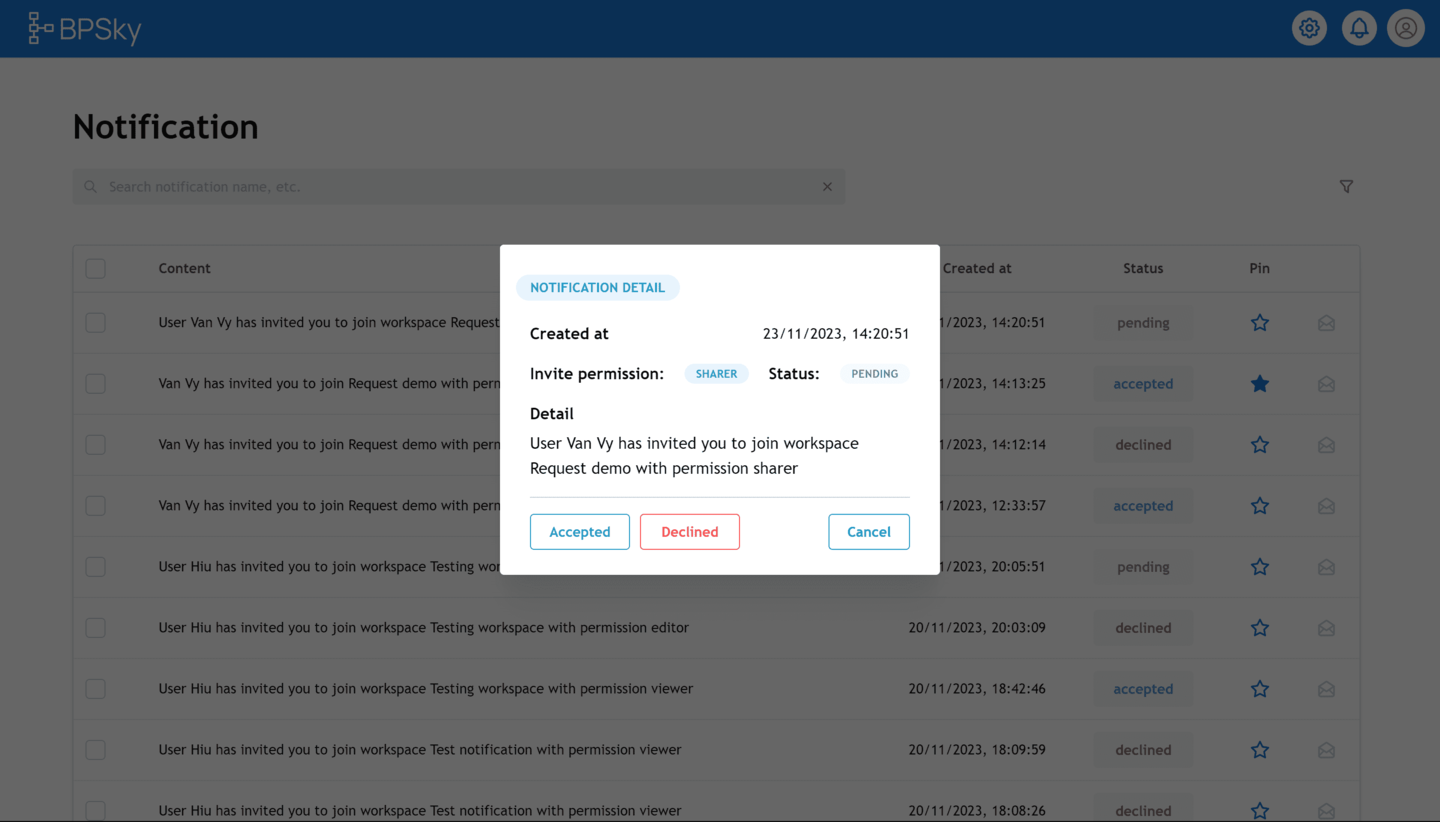
\includegraphics[ width = \linewidth]{Content/Hiện thực hệ thống/documents/Hiện thực giao diện người dùng/images/NotificationDetailModal.png}
    \vspace{0.5cm}
    \caption{Giao diện modal hiển thị thông tin chi tiết của thông báo}
    \label{fig: Giao diện modal hiển thị thông tin chi tiết của thông báo}
\end{figure}

Người dùng có thể xem thông tin chi tiết của mỗi thông báo bằng cách nhấn vào item thông báo tương ứng. Hệ thống sẽ hiển thị giao diện modal như hình \ref{fig: Giao diện modal hiển thị thông tin chi tiết của thông báo}. Tại đây, người dùng có thể xem thông tin chi tiết của thông báo, tùy thuộc vào loại thông báo mà người dùng sẽ có thể tương tác "Approve" - chấp nhận hoặc "Decline" từ chối lời mời được đính kèm trong thông báo. Nếu người dùng muốn đóng modal, người dùng có thể nhấn vào nút "Cancel".